\section{Method}
\label{Method}

To answer our research question we decided to make a simple game, let people play it and ask them questions to obtain the information we were interested in.

%Here you describe what you did and argue for why you want to do it this way and not in some other way. All design choices need to be well motivated.%

\subsection{The Game}
\label{Method_Game}

The game we created required the player to go through four rooms, each time presenting the player with a choice between two doors; one on the right side of the room and one on the left side of the room. After the four rooms, the player ends in a final room with no exits and the game is over. The structure of the rooms can be seen in figure \ref{fig:RoomStructure}.

\begin{figure}[h!]
  \centering
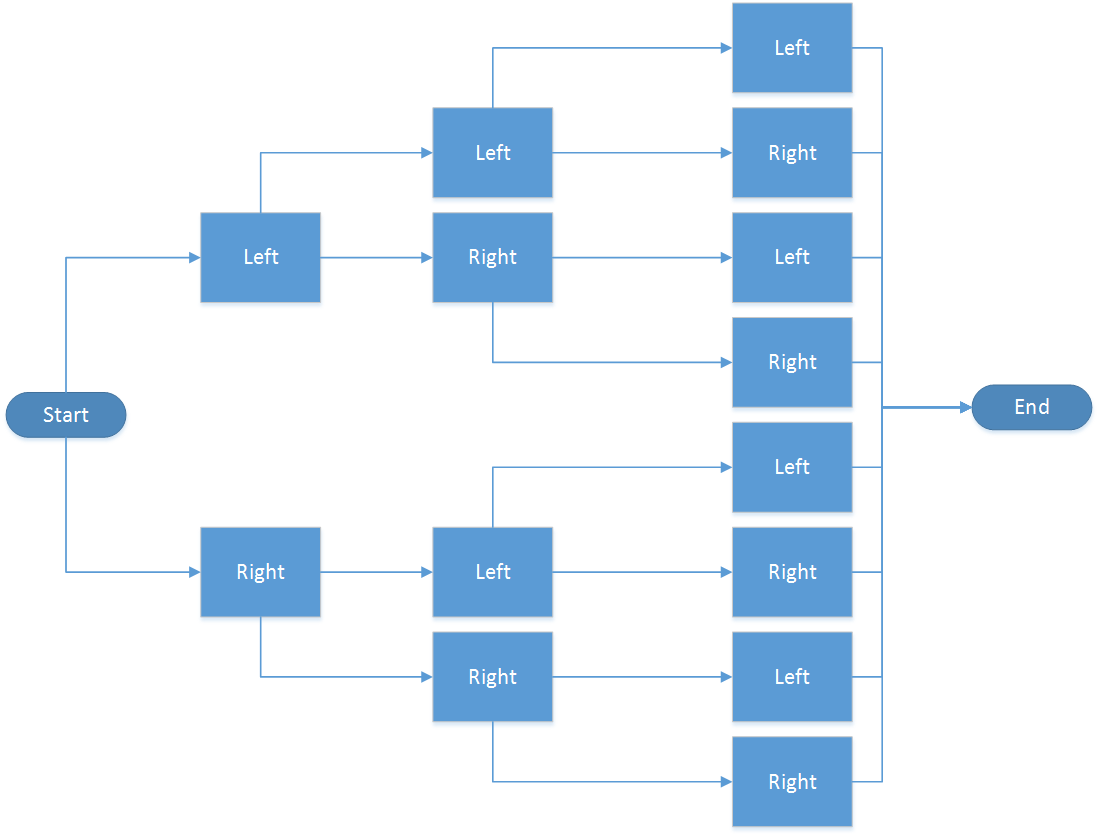
\includegraphics[width=0.5\textwidth]{Parts/RoomStructure}
\caption{The structure of the rooms in the game.}
\label{fig:RoomStructure}
\end{figure}

The first four rooms the player goes through are identical, with an entrance and two exits. The room is square and the walls are grey. There are no objects in the rooms, as we only wanted the narrator to be influencing the player's decision. Had we placed anything else in the rooms, the players might have gotten distracted by it and not paid attention to the narrator.

The last room is different from the others, as it is the last room. This room has the same dimensions and color as the other rooms, but there are no exits, only an entrance. In addition, there is a pile of coins in the middle of the room that represents the player's reward. Attempting to pick the coins up will end the game.

As the player progresses through the rooms, the narrator will speak to them in a way that implies that what the player is experiencing was something that happened in the past (\textit{"Taking the door on the right out of this room would grant him a much higher reward than taking the left door, but he had no way of knowing this."}).

In each room the narrator gives a hint to which door is the better choice, either saying that one would result in a better reward or saying that the other door would decrease the reward. This is part of trying to make the narrator influence the player's decision.

What the narrator says and how he reacts depends on the route the player has chosen. This way, we avoid that some of the script may sound out of place because the player went an unexpected way.

In the last room, the script for the narrator is always the same, no matter the route. We chose to do this, to give the player the feeling that the route they chose did not actually matter, as it actually did not matter. The reward is always the same.

What the player is never told, is that the first four rooms are actually the exact same room. When the player choses an exit, the game records which side they chose and then sends them back to the entrance of the room. This repeats three times, after which the player is let into the final room with the reward. We chose this "one-room-fits-all" method, as there was no need to create fifteen different versions of the exact same room.

While we reuse the same room multiple times, we chose to only have the player go through a few rooms. There were two reasons for this:
\begin{enumerate}
	\item We did not want the player to become bored with walking through rooms, so we kept it to a low number. Adding more rooms would increase the likelihood that the player chose a door just for the sake of doing something different, thereby removing the point of having the narrator affect them.
	\item For every "layer" of rooms, the amount of rooms would be doubled. As we wanted unique script for every possible left/right-combination the player could go, we would need to create more than twice as much audio as we already had for every new layer added.
\end{enumerate}